\section{Results}
\label{sec:results}
% Tables are generated by scripts/make_paper_tables.py (English: runs/experiment_0011; Portuguese and
% cross-lingual: runs/experiment_0014); rerun it after each pull. Partial results carry n=k; empty rows:
% runs not started yet. Text to be written.

\subsection{Main results}
\label{sec:main-results}

\begin{table*}[t]
  \centering\footnotesize\setlength{\tabcolsep}{4pt}
  \textit{(a) English: RoBERTa-large trained on SICK}\\[2pt]
  \begin{tabular*}{\textwidth}{@{\extracolsep{\fill}}lcccccccccc@{}}
\toprule
 & \multicolumn{5}{c}{Accuracy} & \multicolumn{5}{c}{MCC} \\
\cmidrule(lr){2-6}\cmidrule(l){7-11}
System & SICK & AX-b & Break. & Conj. & FraCaS & SICK & AX-b & Break. & Conj. & FraCaS \\
\midrule
\cls{} & 94.3\,{\tiny$\pm$0.4} & 69.1\,{\tiny$\pm$2.5} & \best{95.2}\,{\tiny$\pm$1.1} & 63.0\,{\tiny$\pm$6.2} & 59.6\,{\tiny$\pm$3.3} & 86.0\,{\tiny$\pm$0.9} & 38.2\,{\tiny$\pm$3.7} & 80.3\,{\tiny$\pm$3.0} & 34.2\,{\tiny$\pm$4.5} & 19.6\,{\tiny$\pm$3.8} \\
K-BERT & 93.3$^{\dagger}$\,{\tiny$\pm$0.4} & 66.5$^{\dagger}$\,{\tiny$\pm$1.2} & 95.2\,{\tiny$\pm$0.7} & 57.6\,{\tiny$\pm$4.6} & 58.7\,{\tiny$\pm$1.4} & 83.9$^{\dagger}$\,{\tiny$\pm$0.9} & 33.4$^{\dagger}$\,{\tiny$\pm$1.4} & \best{80.3}\,{\tiny$\pm$2.8} & 22.6$^{\dagger}$\,{\tiny$\pm$4.2} & 16.3$^{\dagger}$\,{\tiny$\pm$1.9} \\
KGAnet & 94.3\,{\tiny$\pm$0.4} & 63.0$^{\dagger}$\,{\tiny$\pm$3.1} & 93.4$^{\dagger}$\,{\tiny$\pm$2.0} & 53.2$^{\dagger}$\,{\tiny$\pm$5.1} & 62.8\,{\tiny$\pm$2.2} & 86.1\,{\tiny$\pm$0.8} & 28.9$^{\dagger}$\,{\tiny$\pm$4.7} & 75.1$^{\dagger}$\,{\tiny$\pm$6.0} & 21.3$^{\dagger}$\,{\tiny$\pm$4.1} & 20.6\,{\tiny$\pm$3.7} \\
KGNLI & \best{94.4}\,{\tiny$\pm$0.2} & 61.4$^{\dagger}$\,{\tiny$\pm$2.1} & 93.0$^{\dagger}$\,{\tiny$\pm$1.5} & 51.6$^{\dagger}$\,{\tiny$\pm$3.3} & 63.9$^{\dagger}$\,{\tiny$\pm$1.3} & \best{86.3}\,{\tiny$\pm$0.5} & 26.4$^{\dagger}$\,{\tiny$\pm$3.0} & 73.8$^{\dagger}$\,{\tiny$\pm$3.9} & 19.0$^{\dagger}$\,{\tiny$\pm$3.4} & 21.4\,{\tiny$\pm$3.3} \\
\model{} & 94.2\,{\tiny$\pm$0.2} & \best{71.6}$^{\dagger}$\,{\tiny$\pm$1.5} & 95.0\,{\tiny$\pm$1.3} & \best{66.7}\,{\tiny$\pm$4.7} & \best{65.7}$^{\dagger}$\,{\tiny$\pm$2.6} & 85.9\,{\tiny$\pm$0.6} & \best{43.1}$^{\dagger}$\,{\tiny$\pm$2.3} & 79.6\,{\tiny$\pm$4.2} & \best{40.1}$^{\dagger}$\,{\tiny$\pm$3.9} & \best{28.2}$^{\dagger}$\,{\tiny$\pm$3.3} \\
\bottomrule
\end{tabular*}

  \vspace{6pt}

  \textit{(b) Portuguese: Albertina-900M trained on InferBR}\\[2pt]
  \begin{tabular*}{\textwidth}{@{\extracolsep{\fill}}lcccccccc@{}}
\toprule
 & \multicolumn{4}{c}{Accuracy} & \multicolumn{4}{c}{MCC} \\
\cmidrule(lr){2-5}\cmidrule(l){6-9}
System & InferBR & ASSIN & ASSIN\,2 & SICK-BR & InferBR & ASSIN & ASSIN\,2 & SICK-BR \\
\midrule
\cls{} & 97.6\,{\tiny$\pm$0.5} & 83.3\,{\tiny$\pm$4.5} & 85.7\,{\tiny$\pm$1.4} & 83.7\,{\tiny$\pm$1.6} & 94.7\,{\tiny$\pm$1.0} & 67.7\,{\tiny$\pm$5.9} & 71.7\,{\tiny$\pm$2.6} & 63.9\,{\tiny$\pm$2.4} \\
K-BERT &  &  &  &  &  &  &  &  \\
KGAnet &  &  &  &  &  &  &  &  \\
KGNLI &  &  &  &  &  &  &  &  \\
\model{} & \best{97.8}\,{\tiny$\pm$0.2} & \best{85.5}\,{\tiny$\pm$2.4} & \best{87.0}$^{\dagger}$\,{\tiny$\pm$0.5} & \best{85.1}$^{\dagger}$\,{\tiny$\pm$0.8} & \best{95.1}\,{\tiny$\pm$0.5} & \best{70.7}\,{\tiny$\pm$3.5} & \best{74.0}$^{\dagger}$\,{\tiny$\pm$1.0} & \best{66.2}$^{\dagger}$\,{\tiny$\pm$1.2} \\
\bottomrule
\end{tabular*}

  \vspace{6pt}

  \textit{(c) Cross-lingual EN$\to$PT: XLM-R-large trained on SICK, Portuguese tests}\\[2pt]
  \begin{tabular*}{\textwidth}{@{\extracolsep{\fill}}lcccccccc@{}}
\toprule
 & \multicolumn{4}{c}{Accuracy} & \multicolumn{4}{c}{MCC} \\
\cmidrule(lr){2-5}\cmidrule(l){6-9}
System & InferBR & ASSIN & ASSIN\,2 & SICK-BR & InferBR & ASSIN & ASSIN\,2 & SICK-BR \\
\midrule
\cls{} & \best{89.9}\,{\tiny$\pm$1.0} & \best{88.8}\,{\tiny$\pm$1.5} & \best{91.3}\,{\tiny$\pm$0.3} & \best{90.7}\,{\tiny$\pm$0.1} & \best{77.0}\,{\tiny$\pm$2.1} & \best{70.8}\,{\tiny$\pm$3.9} & \best{81.7}\,{\tiny$\pm$0.6} & \best{77.0}\,{\tiny$\pm$0.3} \\
K-BERT &  &  &  &  &  &  &  &  \\
KGAnet &  &  &  &  &  &  &  &  \\
KGNLI &  &  &  &  &  &  &  &  \\
\model{} & 88.4$^{\dagger}$\,{\tiny$\pm$1.2} & 86.6$^{\dagger}$\,{\tiny$\pm$2.0} & 91.0\,{\tiny$\pm$0.6} & 90.5\,{\tiny$\pm$0.6} & 73.7$^{\dagger}$\,{\tiny$\pm$2.7} & 66.7$^{\dagger}$\,{\tiny$\pm$3.7} & 81.1\,{\tiny$\pm$1.3} & 76.6\,{\tiny$\pm$1.6} \\
\bottomrule
\end{tabular*}

  \vspace{6pt}

  \textit{(d) Cross-lingual PT$\to$EN: XLM-R-large trained on InferBR, English tests}\\[2pt]
  \begin{tabular*}{\textwidth}{@{\extracolsep{\fill}}lcccccccccc@{}}
\toprule
 & \multicolumn{5}{c}{Accuracy} & \multicolumn{5}{c}{MCC} \\
\cmidrule(lr){2-6}\cmidrule(l){7-11}
System & SICK & AX-b & Break. & Conj. & FraCaS & SICK & AX-b & Break. & Conj. & FraCaS \\
\midrule
\cls{} &  &  &  &  &  &  &  &  &  &  \\
K-BERT &  &  &  &  &  &  &  &  &  &  \\
KGAnet &  &  &  &  &  &  &  &  &  &  \\
KGNLI &  &  &  &  &  &  &  &  &  &  \\
\model{}\textsuperscript{\,$n{=}4$} & \best{87.5}\,{\tiny$\pm$1.5} & \best{68.0}\,{\tiny$\pm$1.3} & \best{94.7}\,{\tiny$\pm$2.6} & \best{65.1}\,{\tiny$\pm$6.0} & \best{66.9}\,{\tiny$\pm$2.2} & \best{72.5}\,{\tiny$\pm$2.1} & \best{38.1}\,{\tiny$\pm$1.1} & \best{79.5}\,{\tiny$\pm$6.8} & \best{39.1}\,{\tiny$\pm$4.7} & \best{28.5}\,{\tiny$\pm$3.0} \\
\bottomrule
\end{tabular*}

  \caption{Main results: accuracy and MCC of \E{} \emph{vs.} $\neg$\E{} ($\times100$), mean and seed
  standard deviation over 10 seeds; best in bold. (c,\,d): zero-shot transfer. $^{\dagger}$Paired Wilcoxon
  $p<0.05$ against \cls{}. \todo{Partial results: $^{n=k}$ marks systems with only $k$ of 10 seeds finished; empty rows
  are still running.}}
  \label{tab:main}
\end{table*}

\subsection{Ablation}
\label{sec:ablation-results}

\begin{table*}[t]
  \centering\footnotesize\setlength{\tabcolsep}{4pt}
  \textit{(a) English: RoBERTa-large trained on SICK}\\[2pt]
  \begin{tabular*}{\textwidth}{@{\extracolsep{\fill}}lccccc@{}}
\toprule
System & SICK & AX-b & Break. & Conj. & FraCaS \\
\midrule
\model{} (full) & 85.9\,{\tiny$\pm$0.6} & 43.1\,{\tiny$\pm$2.3} & 79.6\,{\tiny$\pm$4.2} & 40.1\,{\tiny$\pm$3.9} & 28.2\,{\tiny$\pm$3.3} \\
$-$ conflict & $+$0.2 & $+$2.0 & $+$2.8 & $+$0.4 & \textcolor{red}{$-$0.2} \\
$-$ lexicon & \textcolor{red}{$-$0.4} & $+$0.2 & $+$0.7 & \textcolor{red}{$-$1.6} & $+$0.5 \\
$-$ graph & $+$0.2 & \textcolor{red}{$-$1.8} & $+$1.1 & \textcolor{red}{$-$4.8} & \textcolor{red}{$-$0.3} \\
$-$ coverage & $+$0.2 & \textcolor{red}{$-$6.7$^{*}$} & $+$0.4 & \textcolor{red}{$-$8.5$^{*}$} & \textcolor{red}{$-$9.6$^{*}$} \\
MLP head & \textcolor{red}{$-$0.2} & \textcolor{red}{$-$5.1$^{*}$} & \textcolor{red}{$-$3.2} & \textcolor{red}{$-$11.8$^{*}$} & \textcolor{red}{$-$2.0} \\
\midrule
\cls{} & $+$0.1 & \textcolor{red}{$-$4.9$^{\dagger}$} & $+$0.7 & \textcolor{red}{$-$5.9$^{\dagger}$} & \textcolor{red}{$-$8.6$^{\dagger}$} \\
\bottomrule
\end{tabular*}

  \vspace{6pt}

  \textit{(b) Portuguese: Albertina-900M trained on InferBR}\\[2pt]
  \begin{tabular*}{\textwidth}{@{\extracolsep{\fill}}lcccc@{}}
\toprule
System & InferBR & ASSIN & ASSIN\,2 & SICK-BR \\
\midrule
\model{} (full) & 95.1\,{\tiny$\pm$0.5} & 70.7\,{\tiny$\pm$3.5} & 74.0\,{\tiny$\pm$1.0} & 66.2\,{\tiny$\pm$1.2} \\
$-$ conflict & $+$0.2 & $+$1.0 & $+$0.1 & $+$1.0 \\
$-$ lexicon & \textcolor{red}{$-$0.5} & $+$0.4 & \textcolor{red}{$-$0.3} & $+$0.3 \\
$-$ graph\textsuperscript{\,$n{=}3$} & \textcolor{red}{$-$0.2} & \textcolor{red}{$-$0.2} & \textcolor{red}{$-$0.8} & $+$1.1 \\
$-$ coverage &  &  &  &  \\
MLP head &  &  &  &  \\
\midrule
\cls{} & \textcolor{red}{$-$0.5} & \textcolor{red}{$-$3.0} & \textcolor{red}{$-$2.4$^{\dagger}$} & \textcolor{red}{$-$2.3$^{\dagger}$} \\
\bottomrule
\end{tabular*}

  \vspace{6pt}

  \textit{(c) Cross-lingual: XLM-R-large}\\[2pt]
  \begin{tabular*}{\textwidth}{@{\extracolsep{\fill}}lccccccccc@{}}
\toprule
 & \multicolumn{5}{c}{English tests} & \multicolumn{4}{c}{Portuguese tests} \\
\cmidrule(lr){2-6}\cmidrule(l){7-10}
System & SICK & AX-b & Break. & Conj. & FraCaS & InferBR & ASSIN & ASSIN\,2 & SICK-BR \\
\midrule
\multicolumn{10}{@{}l}{\textit{Train SICK (EN)}} \\
\model{} (full) & -- & -- & -- & -- & -- & 73.7\,{\tiny$\pm$2.7} & 66.7\,{\tiny$\pm$3.7} & 81.1\,{\tiny$\pm$1.3} & 76.6\,{\tiny$\pm$1.6} \\
$-$ conflict & -- & -- & -- & -- & -- & \textcolor{red}{$-$1.9} & \textcolor{red}{$-$4.1} & \textcolor{red}{$-$0.8} & \textcolor{red}{$-$1.1} \\
$-$ lexicon & -- & -- & -- & -- & -- & 0.0 & \textcolor{red}{$-$2.6} & \textcolor{red}{$-$0.2} & 0.0 \\
$-$ graph & -- & -- & -- & -- & -- & \textcolor{red}{$-$0.9} & $+$2.4 & \textcolor{red}{$-$0.5} & \textcolor{red}{$-$0.5} \\
$-$ coverage & -- & -- & -- & -- & -- & \textcolor{red}{$-$0.9} & $+$0.9 & \textcolor{red}{$-$0.8} & 0.0 \\
MLP head & -- & -- & -- & -- & -- & \textcolor{red}{$-$4.0} & \textcolor{red}{$-$3.8} & \textcolor{red}{$-$2.6} & \textcolor{red}{$-$2.6} \\
\midrule
\cls{} & -- & -- & -- & -- & -- & $+$3.3$^{\dagger}$ & $+$4.0$^{\dagger}$ & $+$0.6 & $+$0.3 \\
\midrule
\multicolumn{10}{@{}l}{\textit{Train InferBR (PT)}} \\
\model{} (full)\textsuperscript{\,$n{=}4$} & 72.5\,{\tiny$\pm$2.1} & 38.1\,{\tiny$\pm$1.1} & 79.5\,{\tiny$\pm$6.8} & 39.1\,{\tiny$\pm$4.7} & 28.5\,{\tiny$\pm$3.0} & -- & -- & -- & -- \\
$-$ conflict &  &  &  &  &  & -- & -- & -- & -- \\
$-$ lexicon &  &  &  &  &  & -- & -- & -- & -- \\
$-$ graph &  &  &  &  &  & -- & -- & -- & -- \\
$-$ coverage &  &  &  &  &  & -- & -- & -- & -- \\
MLP head &  &  &  &  &  & -- & -- & -- & -- \\
\midrule
\cls{} &  &  &  &  &  & -- & -- & -- & -- \\
\bottomrule
\end{tabular*}

  \caption{Ablation (binary MCC $\times100$): full model, then mean paired difference to it (decreases in
  red; variants in \cref{sec:ablations}). (c): transfer only. $^{*}$Holm-corrected and $^{\dagger}$uncorrected
  paired Wilcoxon $p<0.05$ against the full model. \todo{Partial results: $^{n=k}$ as in \cref{tab:main}.}}
  \label{tab:ablation}
\end{table*}

\subsection{Error analysis}
\label{sec:error-analysis}

\begin{table}[t]
  \centering\footnotesize
  \setlength{\tabcolsep}{2pt}
  \begin{tabular}{@{}l r ccc@{}}
\toprule
Phenomenon & $n$ & \cls{} & \model{} & $\Delta$ \\
\midrule
\multicolumn{5}{@{}l}{\textit{Categories}} \\
Lexical semantics & 368 & 47.7 & 50.2 & $+$2.5 \\
Predicate--argument structure & 424 & 45.4 & 51.7 & $+$6.3 \\
Logic & 364 & 19.9 & 26.2 & $+$6.3 \\
Knowledge & 284 & 29.5 & 31.5 & $+$2.0 \\
\midrule
\multicolumn{5}{@{}l}{\textit{Largest gains}} \\
Genitives/Partitives & 20 & 57.7 & 90.7 & $+$33.1 \\
Nominalization & 28 & 47.9 & 76.1 & $+$28.2 \\
Morphological negation & 26 & 26.7 & 51.0 & $+$24.3 \\
Temporal & 32 & $-$3.8 & 20.3 & $+$24.1 \\
Double negation & 28 & 16.7 & 39.2 & $+$22.5 \\
Conjunction & 40 & 48.2 & 65.2 & $+$16.9 \\
Coordination scope & 40 & 41.5 & 55.1 & $+$13.6 \\
Anaphora/Coreference & 58 & 37.9 & 50.6 & $+$12.7 \\
\midrule
\multicolumn{5}{@{}l}{\textit{Largest losses}} \\
Restrictivity & 26 & 12.2 & $-$3.7 & \textcolor{red}{$-$15.8} \\
Universal & 18 & 36.3 & 26.2 & \textcolor{red}{$-$10.1} \\
Symmetry/Collectivity & 28 & 34.6 & 25.9 & \textcolor{red}{$-$8.7} \\
Redundancy & 26 & 35.2 & 27.5 & \textcolor{red}{$-$7.7} \\
Downward monotone & 30 & $-$27.6 & $-$33.3 & \textcolor{red}{$-$5.7} \\
\bottomrule
\end{tabular}

  \caption{AX-b by category (bold) and phenomenon, English setting (binary MCC $\times100$, mean over 10
  seeds). $\Delta$: \model{} $-$ \cls{}. Groups with $n<40$ are exploratory.}
  \label{tab:axb-categories}
\end{table}

\subsection{Interpretability}
\label{sec:interpretability}

\begin{figure}[t]
  \centering
  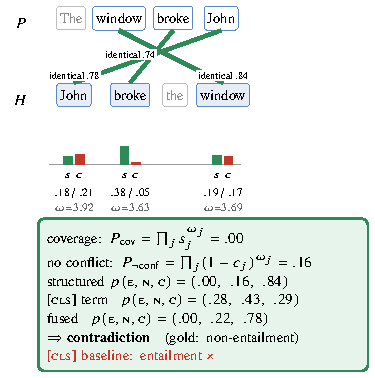
\includegraphics[width=\columnwidth]{figures/explanations/en_cover_1_compact.pdf}
  \caption{A \model{} decision on an AX-b pair that swaps the verb's arguments (RoBERTa-large, seed 1001).
  Lines: alignment (width: attention; label: relation). Bars: support $s_j$, conflict $c_j$, weight
  $\omega_j$. No word is supported in its role, so $\Pcov\approx0$ (not entailed); \cls{} predicts
  entailment.}
  \label{fig:interpretability}
\end{figure}

% Flush the floats before the conclusion (remove once the section has text).
\clearpage
